\documentclass[a4paper,twocolumn]{article}
\usepackage{graphicx}
\usepackage{booktabs}
\usepackage{geometry}
\usepackage{fancyhdr}
\usepackage[skip=2pt]{caption}
\usepackage{indentfirst} 
\usepackage{titling}

% Adjust the margins to use the full space of A4 paper
\geometry{
  a4paper,
  left=17.018mm,
  right=17.018mm,
  top=20.066mm,
  bottom=12.954mm
}

\DeclareCaptionFormat{custom}
{%
    \scriptsize #1 \scriptsize #3
}
\captionsetup{format=custom}


% Set up the header and footer
\fancypagestyle{plain}{
  \fancyhf{}
  \fancyhead[L]{[FM23201]} % Left header
  \fancyfoot[R]{Supervisor[Prof.Makio Ishihara]} % Center footer
  \renewcommand{\headrulewidth}{0pt} % Remove header line
  \renewcommand{\footrulewidth}{0pt} % Remove footer line
}



\pagestyle{plain}
\setlength{\droptitle}{-4em}     % Eliminate the default vertical space
\addtolength{\droptitle}{-2pt}   % Only a guess. Use this for adjustment
\title{\textbf{The Development of Haptic Feedback Data Glove for Enhancing Immersion in VR Experiences}}
\author{\small{Korntawat Witchuvanit (Computer Science and Engineering)}}
\date{\vspace{-3em}}

\begin{document}
\small
\maketitle

% Redefine the section command to use a smaller font size and reduce spacing
\makeatletter
\renewcommand\section{\@startsection{section}{1}{\z@}%
  {-1.0ex \@plus -0.5ex \@minus -.2ex}%  % Adjust the spacing before the section title
  {0.3ex \@plus 0.2ex}%  % Adjust the spacing after the section title
  {\normalfont\small\bfseries}}
\makeatother



\section{Introduction}
Virtual reality (VR) enhances immersion through multi-sensory feedback, with haptic feedback bridging the virtual and physical worlds. While traditional VR focuses on visual and auditory cues, rendering virtual textures through touch remains challenging. Many methods use hand-held devices, restricting natural hand movements. This research introduces a haptic glove with flex sensors, an MPU, and a coin motor, enabling texture perception at three vibration granularities, offering a more intuitive and immersive tactile experience in VR.

\section{Previous Methods}
Deep-Texture[1] is a foldable device for rendering shape and texture in VR. Using a linear resonant actuator and a 1-bar mechanism, it delivers lightweight, effective haptic feedback. Pilot tests show improved user experience. The next study[2] introduced audio-based vibrotactile feedback in VR, enhancing realism and user experience. Multimodal feedback was preferred, supporting immersive interactions. Future work will explore real-time synthesis based on virtual object properties.

\section{Proposed Method}
Our proposed device is a sensor-equipped glove designed to enable finger tracking while delivering realistic haptic feedback. The glove integrates multiple key components to enhance interaction and immersion. Flex sensors are attached to each finger, allowing the system to detect bending and movement, accurately measuring the degree of flexion to interpret finger gestures in real time. An Inertial Measurement Unit (IMU), specifically an MPU, is embedded to track hand orientation, acceleration, and rotation, enabling motion capture and seamless interaction within virtual environments. Micro-vibration motors are placed within the glove to enhance tactile realism and provide haptic feedback, generating subtle vibrations that simulate textures during virtual interactions.

\section{Experimental Setup}
We involved six male participants in their 20s, who conducted two experiments to evaluate haptic feedback perception. The haptic feedback in this experiment were generated using the Pulse Width Modulation (PWM) method at three different cycle rates: 20 cycles, 50 cycles, and 100 cycles, each representing a distinct texture sensation. The experimental setup involves the following steps: \par
In the first experiment, participants conducted a blind test to distinguish between three different haptic feedback. Before starting, they were introduced to all three granularities. A white 3D plane then appeared in the virtual environment, randomly generating one of the granularities upon contact with the virtual hand. Participants identified the perceived granularity, repeating the process 15 times to assess their ability to differentiate between them.\par
The second experiment explored the relationship between haptic feedback granularities and texture perception. Participants interacted with a textured 3D plane (brick, grass, or marble), each generating three different haptic feedback granularities. After experiencing all three granularities for a given texture, they selected the one they felt best matched the material before proceeding to the next texture.\par
After completing an evaluation questionnaire after the experiments. 					

\section{Results}
The results indicate that in the blind test involving three haptic feedback granularities, participants were able to distinguish between the lowest granularity (20 cycles) and the highest granularity (100 cycles), as shown in Fig. 1. However, the scores for the middle granularity (50 cycles) were similar to those of the lowest granularity. Some participants noted that 'the glove is too big for my hand, making it difficult to identify the granularities accurately.' This may be due to the use of a standard glove with an attached component, which cannot be adjusted to fit every hand.\par
the result of second experiment as shown in fig.2. For Marble which represent the smoothest material is compatible with 100 cycle while the grass is likely to 50 duty cycle and for the last one that represent the least smoothness is 20 and 50 duty cycle is equal

\begin{figure}[h]
  \centering
  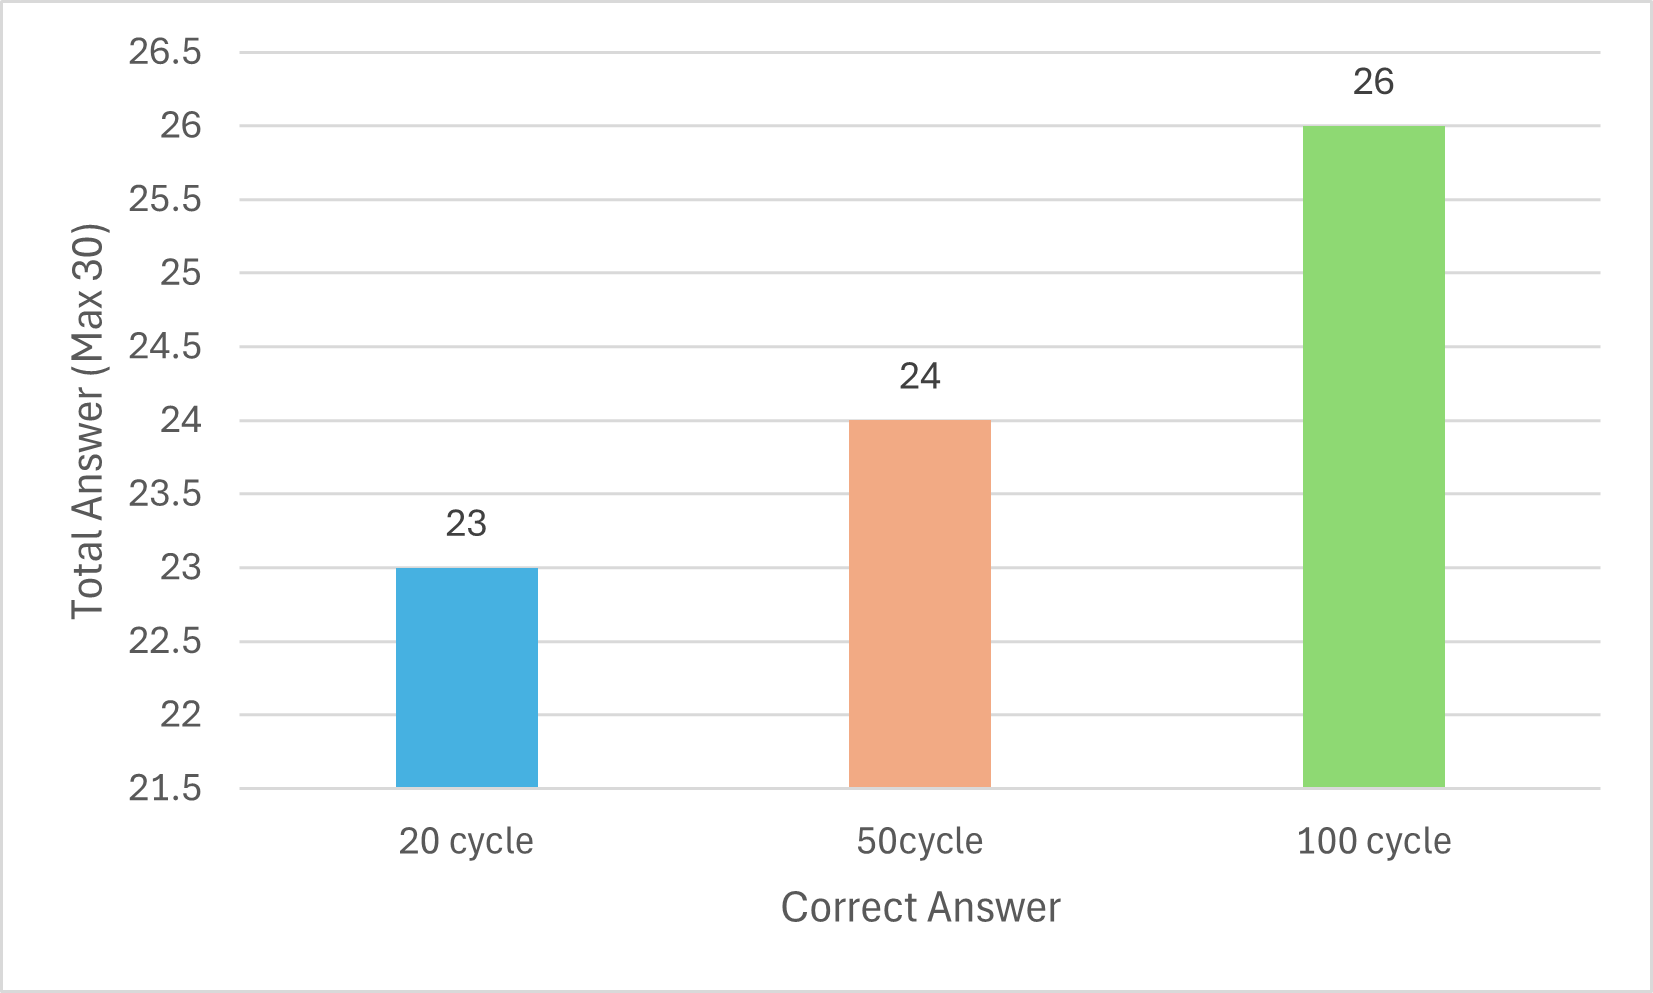
\includegraphics[width=0.35\textwidth]{./Fig/Blind_Test_graph.png}
  \caption{{Result of First Experiment}}
  \label{fig1}
  \vspace{0.1cm}
  \centering
  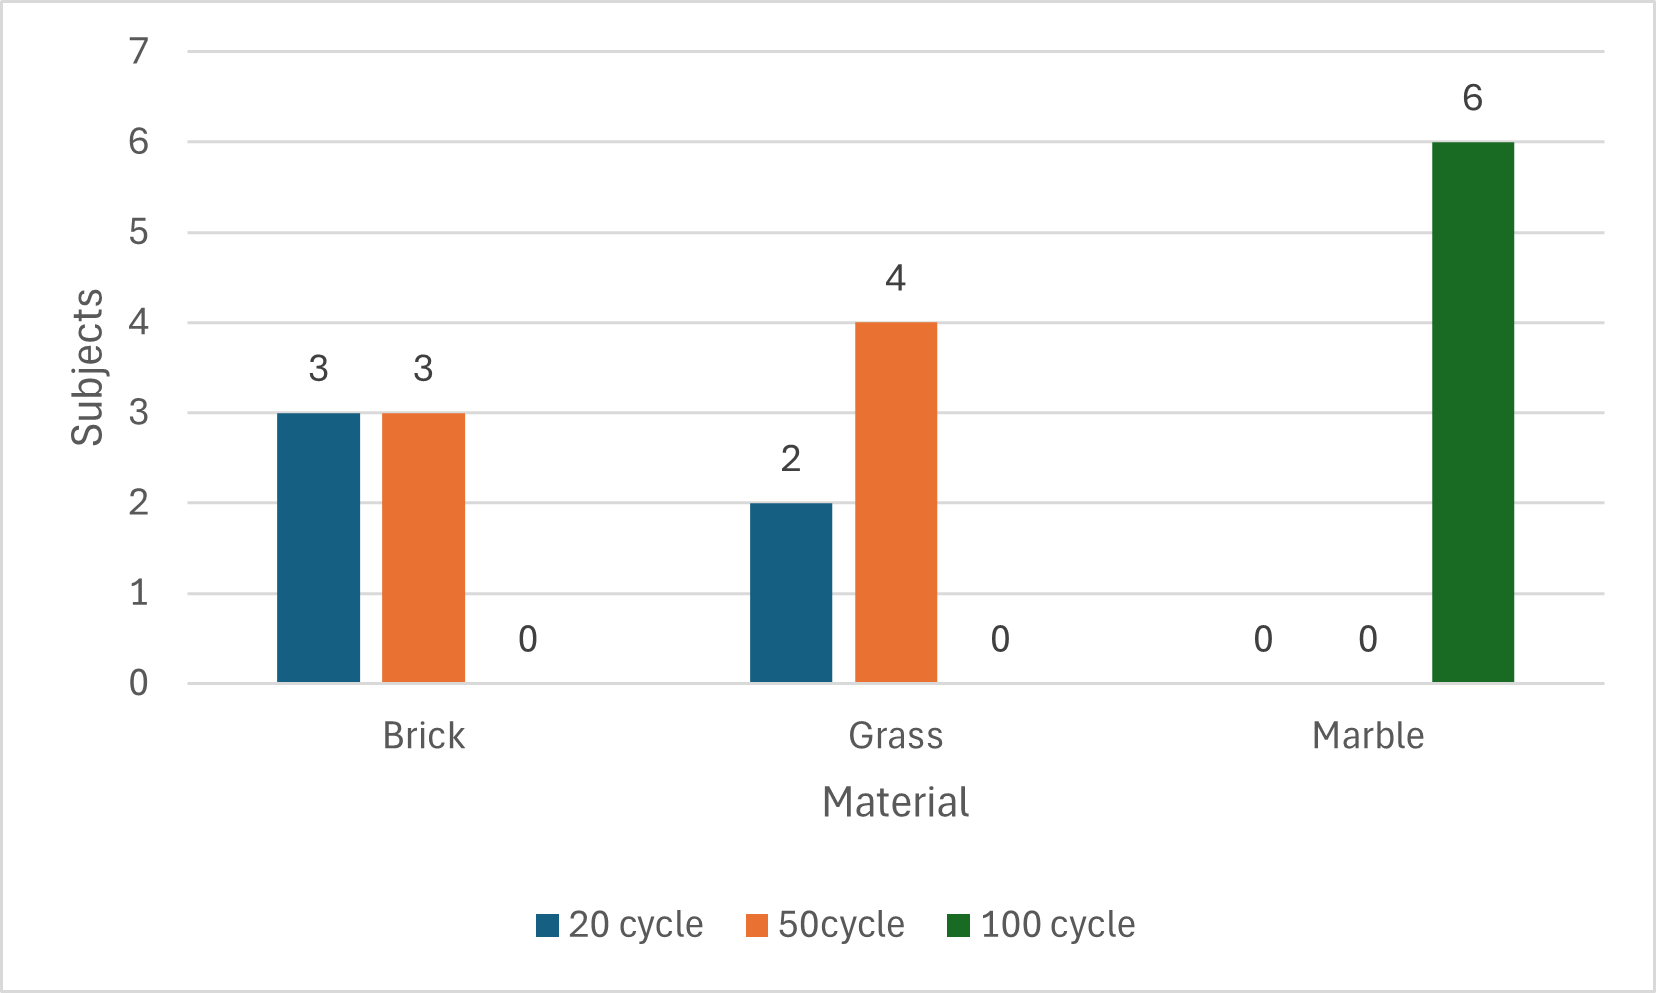
\includegraphics[width=0.35\textwidth]{./Fig/Select_Cycle_graph.png}
  \caption{{Result of Second Experiment}}
  \label{fig2}
\end{figure}


\section{Conclusion}
The results show that participants could distinguish between the lowest (20 cycles) and highest (100 cycles) haptic granularities, but not the middle (50 cycles), possibly due to glove fit issues. Additionally, material smoothness influenced duty cycle compatibility, with marble aligning with 100 cycles, grass with 50 cycles, and the roughest material showing no clear preference between 20 cycles and 50 cycles. These findings highlight the role of both granularity and material in haptic feedback effectiveness.
\begin{thebibliography}{99}
\scriptsize
    \bibitem{sdn1} Y. Sung, D. Kwak, T. Kim, W. Woo and S. H. Yoon, "Deep-Texture: A Lightweight Wearable Ring for Shape and Texture Rendering in Virtual Reality," 2024 IEEE Conference on Virtual Reality and 3D User Interfaces Abstracts and Workshops (VRW), Orlando, FL, USA, 2024, pp. 911-912
    \bibitem{sdn2} Oscar Ariza, Felix Steiner, André Zenner, and Frank Steinicke. 2023. Audio-based Vibrotactile Feedback in Multimodal VR Interactions. In Proceedings of the 29th ACM Symposium on Virtual Reality Software and Technology (VRST '23). Association for Computing Machinery, New York, NY, USA, Article 43, 1–2.
\end{thebibliography}

\end{document}


% Ref. for Figures and Tables
% \begin{table}[ht]
%     \centering
%     \begin{tabular}{|c|c|c|}
%         \hline
%         Condition & Score & Comment \\
%         \hline
%         A & 5.0 & Good \\
%         B & 3.8 & Average \\
%         C & 2.5 & Poor \\
%         \hline
%     \end{tabular}
%     \caption{Experimental Results}
%     \label{tab:results}
% \end{table}

% \begin{figure}[ht]
%     \centering
%     \includegraphics[width=0.8\linewidth]{example-image} % Replace with your figure
%     \caption{Experimental Result 1}
%     \label{fig:result1}
% \end{figure}